%%%%%%%%%%%%%%%%%%%%%%%%%%%%%%%%%%%%%%%%%%%%%%%%%%%%%%%%%%%%%

\mainmatter
\setcounter{page}{1}

\lectureseries[\course]{\course}

\auth[\lecAuth]{Lecturer: \lecAuth\\ Scribe: \scribe}
\date{November 10, 2009}

\setaddress

% the following hack starts the lecture numbering at 13
\setcounter{lecture}{12}
\setcounter{chapter}{12}

\lecture{Convergence \& Consistency}

\section{Prediction Review}
In Lecture 11 (\ref{eq:error}) showed that the prediction error is
\begin{align*}
\epsilon(t,\theta) &= H_0^{-1}(q)[y(t)-G_0(q)u(t)] \\
\hat{\theta} &= \arg\min_\theta\frac{1}{N}\sumt\epsilon^2(t,\theta)
\end{align*}

In Table \ref{tab:models} we looked at different model strutures to parameterize $G_\theta$ and $H_\theta$, some of which were ARX, ARMAX, OE, BJ, PEM. We saw that conventional least squares is equivalent to using PEM+ARX.  The structural parameters for these models were given as $n_a$, $n_b$, $n_c$, $n_d$, $n_f$ and $n_k$.

\section{Convergence \& Consistency for PEM Model}
This section corresponds to Chapter 8 in Ljung. See Figure \ref{fig:13overview} to see how models are typically used and validated. If the model is not validated then we can go back and modify our experiments to collect new or more data. The model $M(\theta)$ needs prior assumptions about what noise model structure will be used and the order of the noise/system. Optimization can be performed using conventional, time-weighted or constrained least squares approaches or even quadratic programming. When attempting to validate a model we typically assume that $u(t)\perp e(t)$. The validation process usually involves checking to see if $e(t)$ or $\epsilon(t,\theta)$ are white noise. If they are white it means that we have extracted all of the useful information out of the system and the model is a good fit, see \S\ref{sec:generalpredictor} for more details.

\begin{figure}[ht!]
	\centering
	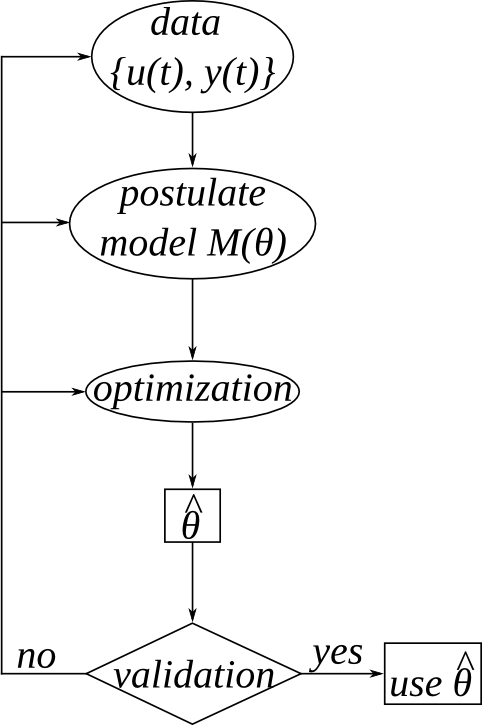
\includegraphics[width=.5\textwidth]{images/13overview}
	\caption{Overview of identifying parameter estimates.}
	\label{fig:13overview}
\end{figure}

A model is consistent if $\mathcal{S}\in\mathcal{M}$. A model converges if $\lim_{N\to\infty}\hat{\theta}^N = \theta_0$ w.p. $1$. We will use the steps in Figure \ref{fig:13overview} to look at these properties of models. First we have to make some assumptions.

\subsection{Assumptions on Data}
\label{sec:14data}
This section will address the assumptions on the data collected, namely $\{u(t),y(t)\}$. Recall from \S\ref{sec:upersistent} that for a least squares estimate the input signal must be persistently exciting so that $R^{-1}(N)$ will exist. For more general cases of we will look at the input and output as combinations of filters with reference signals and errors such that
\begin{align*}
y(t) &= \sumk d_1(k)R(t-k) + \sumk d_2(k)e(t-k) \\
u(t) &= \sumk d_3(k)R(t-k) + \sumk d_4(k)e(t-k)
\end{align*}
$\{R(t)\}$ is a bounded, deterministic signal and $\{e(t)\}$ is an independent, random variable with variance $E\{e(t)\} = 0$, covariance $E\{e^2(t)\}<C_2<\infty$ and fourth moment $E\{e^4(t)\}<C_4<\infty$. The result of looking at the input and output signals in this fashion is that a family of transfer functions describes the data where
$$\sumk d_i(k)q^{-k}, \qquad i=1,2,3,\ldots$$
are all BIBO stable (see \S\ref{sec:bibostability}). We also need to assume that $\{u(t)\}$ and $\{y(t)\}$ are jointly quasi-stationary (\S\ref{def:quasistationary}) so that we can still find the spectral densities and covariance functions because the variance properties don't change over time. This generality lets us examine systems like open-loop controllers such as shown in Figure \ref{fig:13openloop}. In that case a lot of the transfer function terms will go to zero, or $d_i(k)\to0$. For feedback controllers with a reference point like that in Figure \ref{fig:13feedback} we have that many of the transfer function terms are non-zero but we use the same tools to analyze both types of systems.

\begin{figure}[ht!]
  \centering
  \subfloat[Open-loop.]{
    \label{fig:13openloop}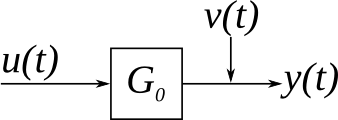
\includegraphics[width=0.4\textwidth]{images/13openloop}
  } \hfill
  \subfloat[Feedback.]{
    \label{fig:13feedback}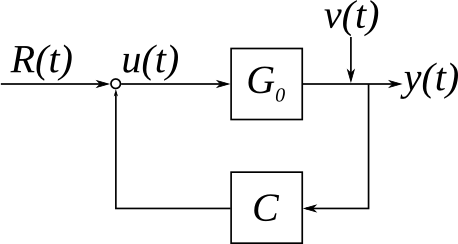
\includegraphics[width=0.4\textwidth]{images/13feedback}
  } \hfill
  \caption{Block diagrams for open-loop and feedback controllers.}
  \label{fig:13blocks}
\end{figure}

\subsection{Assumptions on System}
This section will address the assumptions that need to be made about the system so that a model can be generated. Remember that the model does not need to capture all of the information about the system it just needs to be a simplified version of the system that can be used to describe the important parameters of the system. To that end we will assume that there exists parameters $\theta$ such that
$$\mathcal{S}=\mathcal{M}(\theta_0)$$
and we will refer to this as $\mathcal{S}\in\mathcal{M}$.

\subsection{Assumptions on Optimization}
This section will address the assumptions about optimizing the model so that the parameters estimated more closely reflect the actual system behavior. We will assume that the noise is Gaussian such that
$$e(t)\sim\mathcal{N}(0,\lambda), \qquad E\{e^2(t)\}=\lambda$$
We don't \textit{have} to make this assumption but it makes some of the following derivations easier to compute. With this assumption we get that
$$\thetan = \arg\min_\theta \onen\sumt \epsilon(t,\theta)^2$$
will be the maximum likelihood estimate, e.g., $\thetan$ will have the smallest variance. In addition we will also sometimes use the assumptions that
\begin{align}
\label{eq:13filter}
\thetan &= \onen\sumt\epsilon_F(t,\theta)^2, \qquad \text{where } \epsilon_F(t,\theta)=F(q)\epsilon(t,\theta) \\
\label{eq:13tw}
\thetan &= \onen\sumt\left[w(t)\epsilon_F(t,\theta)\right]^2 \\
\label{eq:13mv}
\thetan &= \onen\sumt\text{tr}\{\epsilon(t,\theta)\Lambda\epsilon^T(t,\theta)\}
\end{align}
(\ref{eq:13tw}) is the time-weighted least squares estimate and (\ref{eq:13mv}) is the multi-variable version. All of these expressions are $2$-norm minimizations. Notice that if $\epsilon$ is a scalar then $\Lambda$ is a scalar and can be moved outside of the trace and we get back to the previous definitions. However, if we look at the case where $\epsilon$ is two variables then we have
$$\underbrace{\epsilon(t,\theta)}_{1\times2}\underbrace{\Lambda}_{2\times2}\underbrace{\epsilon^T(t,\theta)}_{2\times1}\Rightarrow1\times1$$
This still results in a scalar value but $\Lambda$ can be seen to be a scaling matrix that, for example, can normalize measurements made when one is in feet and the other is in miles.

\section{Filtering the Prediction Error}
Why would we want to filter the prediction error as in (\ref{eq:13filter})? Figure \ref{fig:13errorfilter} shows that $H_\theta$ is a noise filter that can be set to $1$. Then, we can use the filter $F(q)$ to make the prediction error be as close as possible to white noise and it will play the role of noise filter (see \S\ref{sec:generalpredictor} for more details about why the output error should be white noise).

\begin{figure}[ht!]
	\centering
	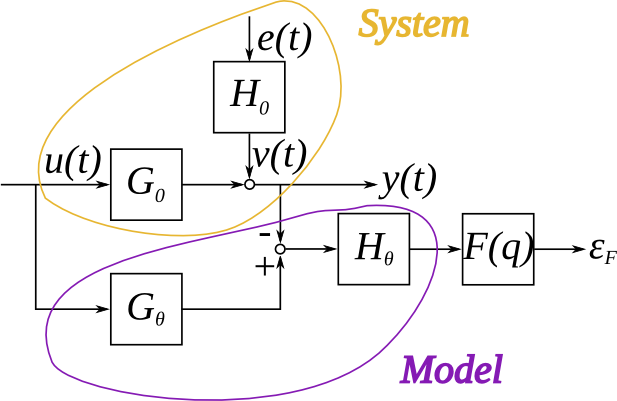
\includegraphics[width=.5\textwidth]{images/13errorfilter}
	\caption{Example of prediction error filter in block diagram.}
	\label{fig:13errorfilter}
\end{figure}

Another reason to filter the prediction error is in the case where $\mathcal{S}\notin\mathcal{M}$ and we can use $F(q)$ to emphasize certain frequency ranges, for example as a band-pass filter.

Now, with these assumptions we can look at what happens to the estimated parameter as more and more data is collected.

\section{Convergence Result}
\label{sec:convergence}
Let
$$\thetan = \arg\min_\theta V_N(\theta,Z^N) = \onen\sumt\epsilon^2(t,\theta)$$
where $\theta$ is the parameter and $Z^N$ is the input and output data. Let $\mathcal{M}$ be a model set with a parameter set $\Theta$ that is uniformly stable and let $Z^\infty$ satisfy the assumptions mentioned in this Lecture. Then
\begin{align}
\label{eq:13convergence}
\sup_{\theta\in\Theta}\left|V_N(\theta,Z^N)-\bar{V}(\theta)\right| \to 0 \text{ w.p. } 1
\end{align}
where $\bar{V}(\theta)=\bar{E}\{\epsilon^2(t,\theta)\}$. Note that the variance of the parameter estimate is then
$$\lim_{N\to\infty}\onen\sumt\epsilon^2(t,\theta) = R_\epsilon(\tau=0) = E\{\epsilon^2(t,\theta)\}$$
(\ref{eq:13convergence}) means that the stochastic variable $V_N(\theta,Z^N)$ converges to $\bar{V}(\theta)$ and note that $\bar{V}(\theta)$ does not depend on the data as $N\to\infty$.

We then have that if
$$\thetan = \arg\min_\theta V_N(\theta,Z^N)$$
then
$$\lim_{N\to\infty}\thetan = \theta^\ast \text{ w.p. } 1$$
where $\theta^\ast = \arg\min_\theta \bar{V}(\theta)$ and $\bar{V}(\theta) = E\{\epsilon^2(t,\theta)\}$. Again, as $N\to\infty$ we have that $\hat{\theta}$ is independent of the data.

Obviously, if we have that $\mathcal{S}\in\mathcal{M}$ then $\theta^\ast=\theta_0$. If $\mathcal{S}\notin\mathcal{M}$ then $\thetan\to\theta^\ast$ but $\theta^\ast\neq\theta_0$. Instead, we will end up with a biased estimate if the actual system is not in our model set. See Figure \ref{fig:13bias}.

\begin{figure}[ht!]
	\centering
	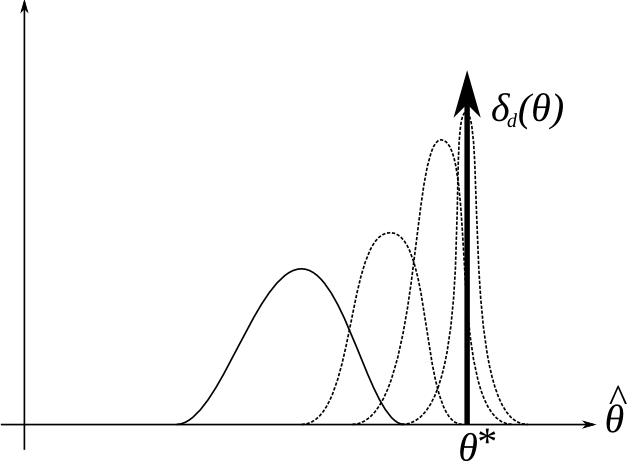
\includegraphics[width=.4\textwidth]{images/13bias}
	\caption{Biased parameter estimate.}
	\label{fig:13bias}
\end{figure}

\begin{example}
\label{ex:convergence}
Let the system and model be stable with the system described by
\begin{align*}
\mathcal{S}: G_0(q) = \frac{b_0q^{-1}}{1+a_1q^{-1}}, \qquad H_0(q)=\frac{1+c_0q^{-1}}{1+a_0q^{-1}}
\end{align*}
and the model has the condition that there exists $\theta_0$ such that $\mathcal{M}(\theta_0) = \mathcal{S}$. The model that fits this best (see Table \ref{tab:models}) is the ARMAX model given by
\begin{align*}
G_\theta(q) = \frac{bq^{-1}}{1+aq^{-1}}, \qquad H_\theta(q)=\frac{1+cq^{-1}}{1+aq^{-1}}
\end{align*}
and the parameter is $\theta=\left[\begin{array}{c c c} a & b & c \end{array}\right]$. We also have that $n_a=1$, $n_b=1$, $n_c=1$ and $n_k=1$ so we would call \texttt{theta = armax([y u],[1 1 1 1])} in \textsc{Matlab}. For this example we are using $u(t)$ as white noise with unit variance.

We know from earlier in this lecture that
$$\lim_{N\to\infty}\thetan = \theta_0 \text{ w.p. } 1$$
But, ARMAX requires non-linear optimization and it is possible to get stuck in a local minima when searching for the parameter estimate. However, if we use an ARX model then we get
\begin{align*}
G_\theta(q) = \frac{bq^{-1}}{1+aq^{-1}}, \qquad H_\theta(q)=\frac{1}{1+aq^{-1}}
\end{align*}
and $\theta=\left[\begin{array}{c c} a & b \end{array}\right]$. This means we can use linear solvers and will be estimating a lower-dimensional parameter and will not get to $\theta_0$. But,
$$\lim_{N\to\infty}\thetan = \theta^\ast \text{ w.p. } 1$$
What is $\theta^\ast$? Does it converge to the the true parameter, $\theta_0$?

We can re-write the system as
\begin{align*}
y(t) &= \frac{b_0q^{-1}}{1+a_1q^{-1}}u(t) + \frac{1+c_0q^{-1}}{1+a_0q^{-1}}e(t) \\
y(t) &= -a_0y(t-1) + b_0u(t-1) + \underbrace{e(t) + c_0e(t-1)}_{w(t)}
\end{align*}
Now, we have the system and model as
\begin{align*}
\mathcal{S}: y(t) &= \vp^T(t)\theta_0+w(t), \qquad \theta_0=\left[\begin{array}{c}b_0\\a_0\end{array}\right], \qquad \vp^T(t) = \left[\begin{array}{c c} u(t-1) & -y(t-1) \end{array}\right] \\
\mathcal{M}: y(t) &= \vp^T(t)\theta+\epsilon(t,\theta), \qquad \theta=\left[\begin{array}{c}b\\a\end{array}\right]
\end{align*}
The parameter estimate is
$$\hat{\theta} = \arg\min_\theta\onen\sumt\epsilon^2(t,\theta)$$
For the least squares estimate to work we need
\begin{itemize}
\item $u\perp v$
\item $\{u(t)\}$ persistently exciting
\item $\vp\perp w\Rightarrow\{w(t)\}$ must be white noise
\end{itemize}
But, we have that $e(t)$ is correlated with $e(t-1)$ because of the time-shift so $\vp(t)$ is also correlated with $w(t)$ and the estimate $\theta^\ast\neq\theta_0$.

We can find the parameter estimate and prediction error as
\begin{align*}
\theta^\ast &= \arg\min_\theta\bar{V}(\theta) \\
\bar{V}(\theta) &= E\{\epsilon^2(t,\theta)\} \\
\epsilon(t,\theta) &= H_\theta^{-1}(q)[y(t)-G_\theta(q)u(t)] \\
&= (1+aq^{-1})\left[y(t) - \frac{bq^{-1}}{1+aq^{-1}}u(t)\right] \\
&= (1+aq^{-1})y(t) - bq^{-1}u(t) \\
&= y(t)+ay(t-1)-bu(t-1) \\
\theta &= \left[\begin{array}{c} b \\ a \end{array}\right]
\end{align*}
We find $\bar{V}(\theta)$ using
\begin{align*}
\bar{V}(\theta) &= \bar{E}\{[y(t)+ay(t-1)-bu(t-1)][y(t)+ay(t-1)-bu(t-1)]\} \\
&= (1+a^2)R_y(0) + 2aR_y(1) + b^2 - 2bR_{yu}(1) - 2abR_y(0)
\end{align*}

From here we set up four equations to determine the four unknowns while recalling that for this example $u(t)$ and $e(t)$ are white noise.
\begin{align*}
R_{yu}(0) + a_0R_{yu}(1) &= b_0R_u(1) = 0 \\
R_{yu}(1) + a_0R_{yu}(0) &= b_0R_u(0) = b_0 \\
R_{ye}(1) + a_0\underbrace{R_{ye}(-1)}_{=0} &= \underbrace{R_e(0)}_{=1} + c_0\underbrace{R_e(1)}_{=0} \\
R_y(1) + a_0R_y(0) &= b_0R_{yu}(0) + c_0R_{ye}(0) \\
\Rightarrow R_{yu}(0) &= 0 \\
R_{yu}(1) &= b_0 \\
R_{ye}(0) &= 1 \\
R_y(1) &= c_0-a_0R_y(0) = c_0-a_0R_0
\end{align*}
Note that $R_{yu}(1)$ is the first impulse response coefficient and $R_{ye}(0)=1$ because $H_0$ is monic. This lets us solve for $\bar{V}(\theta)$ as
$$\bar{V}(\theta) = (1+a^2-2aa_0)R_0+2ac_0 + b^2 - 2bb_0$$
We want to minimize this with respect to both $a$ and $b$ and use
\begin{align*}
\left.\frac{\partial\bar{V}(\theta)}{\partial a}\right|_{a=a^\ast} &= 0 \Rightarrow 2(a^\ast-a_0)R_0+2c_0=0 \\
\left.\frac{\partial\bar{V}(\theta)}{\partial b}\right|_{b=b^\ast} &= 0 \Rightarrow 2(b^\ast-b_0)=0
\end{align*}
which yields
\begin{align*}
b^\ast &= b_0 \\
a^\ast &= a_0-\frac{c_0}{R_0}
\end{align*}
Since the ARX model ignored the $c_0$ term in the real system we are getting bias because we are not estimating that parameter. All of this yields the relation
\begin{align*}
\boxed{\min_\theta\bar{V}(\theta) = 1+a_0^2-\frac{c_0^2}{R_0^2}}
\end{align*}
The real pole, $a_0$, is being biased by the noise, $c_0$.

If we substitute $a_0$ and $b_0$ into $\theta$ then we get
$$\left.\bar{V}(\theta)\right|_{\theta=\left[\begin{array}{c}b_0\\a_0\end{array}\right]} = 1+c_0^2 > 1+c_0^2-\frac{c_0^2}{R_0^2}$$
so the biased estimate is better at minimizing the prediction error but might not be so good to use for controlling the system.
$\lozenge$
\end{example}

%%%%%%%%%%%%%%%%%%%%%%%%%%%%%%%%%%%%%%%%%%%%%%%%%%%%%%%%%%%%%